\section{Results and Discussion}
\label{sec:results}

We evaluate the numerical accuracy, algorithmic efficiency, and physical implications of our optimization framework across a series of validation benchmarks and network stress sweeps on the IEEE 30-bus system.

\subsection{Solver Validation}

Table~\ref{tab:validation} compares our custom solvers (the primal active-set QP solver and the lambda-iteration bisection solver) against the CVXPY reference solver with the Clarabel backend across three standard benchmarks: uncongested DC-OPF (base case), congested DC-OPF (line ratings scaled to $0.75\times$), and Economic Dispatch (ED base).

\begin{table}[htbp]
\centering
\caption{Solver comparison: cost, primal/dual error vs.\ reference, KKT stationarity residual, and iteration counts (from default start and non-optimal start).}
\label{tab:validation}
\begin{tabular}{llrrrrrr}
\toprule
Solver & Scenario & Cost (\$/h) & $\max|\Delta x|$ & $\max|\Delta\lambda|$ & KKT res. & Iters & Iters (non-opt) \\
\midrule
reference & base & 565.21 & 0.00e+00 & 0.00e+00 & 8.31e-09 & 7 & --- \\
reference & rate\_0.75 & 565.97 & 0.00e+00 & 0.00e+00 & 2.06e-07 & 9 & --- \\
reference & ed\_base & 565.21 & 0.00e+00 & 0.00e+00 & 7.45e-07 & 6 & --- \\
active\_set & base & 565.21 & 4.27e-08 & 8.59e-10 & 2.40e-11 & 1 & 13 \\
active\_set & rate\_0.75 & 565.97 & 9.80e-06 & 8.86e-06 & 9.55e-12 & 9 & 14 \\
active\_set & ed\_base & 565.21 & 8.77e-07 & 4.00e-10 & 2.40e-11 & 1 & 11 \\
lambda\_iter & ed\_base & 565.21 & 8.77e-07 & 4.31e-10 & 5.07e-09 & 33 & --- \\
\bottomrule
\end{tabular}
\end{table}

Across all scenarios, our active-set solver agrees with the reference solution to high numerical precision. In the uncongested base case and ED problem, the active-set solver achieves primal errors $\max |\Delta x| \le 4.27 \times 10^{-8}$ and dual errors $\max |\Delta \lambda| \le 8.59 \times 10^{-10}$, with KKT stationarity residuals on the order of $10^{-11}$. In the congested scenario (ratings $\times 0.75$), the active-set solver matches the reference solution with primal deviation $\max |\Delta x| = 9.80 \times 10^{-6}$, dual deviation $\max |\Delta \lambda| = 8.86 \times 10^{-6}$, and KKT residual $9.55 \times 10^{-12}$. The lambda-iteration solver solves the ED problem to $\max |\Delta x| = 8.77 \times 10^{-7}$ in 33 bisection iterations.

When initialized from the default \texttt{feasible\_start()} point, the base DC-OPF and ED problems converge in a single iteration because the initial point is already the unconstrained global minimizer. To evaluate the active-set solver's ability to perform active-set identification from a distant state, we compute non-optimal feasible starting points via linear programming ($\min -g^T x$). From these non-optimal points, the active-set solver takes 13 iterations on the base case, 14 iterations on the $0.75\times$ congested case, and 11 iterations on ED, systematically adjusting the working set until optimality is proven.

\subsection{Price Sensitivity and +1~MW Verification}

To confirm the economic interpretation of the equality dual multipliers as Locational Marginal Prices, we apply a $+1.0\text{ MW}$ active load increase at buses 8 and 30 in the base case using our active-set solver (\texttt{results/plus1mw.csv}). In both cases, the point derivative LMP reported by the solver is $\lambda_k = 3.789196\text{ \$/MWh}$, while the finite-difference cost increase is $\Delta q^* = 3.792292\text{ \$}$.

The observed discrepancy of $\Delta q^* - \lambda_k = +0.003096\text{ \$}$ perfectly matches the theoretical second-order Taylor expansion term:
\begin{equation}
    \frac{1}{2} \left( \sum_{i=1}^6 \frac{1}{2 c_i} \right)^{-1} (\Delta d)^2 = \frac{1}{2} (0.006191) (1.0)^2 = +0.003096\text{ \$}
\end{equation}
This confirms that the dual multipliers represent exact marginal prices at the optimum, and that the finite-difference difference is purely attributable to generator quadratic cost curvature rather than dual multiplier error.

\subsection{Price vs.\ Demand (Economic Dispatch)}

Figure~\ref{fig:price_demand} presents the system marginal price $\lambda$ as total demand is scaled from $94.60\text{ MW}$ to $331.10\text{ MW}$ (0.50 to 1.75 load scale factor).

\begin{figure}[htbp]
\centering
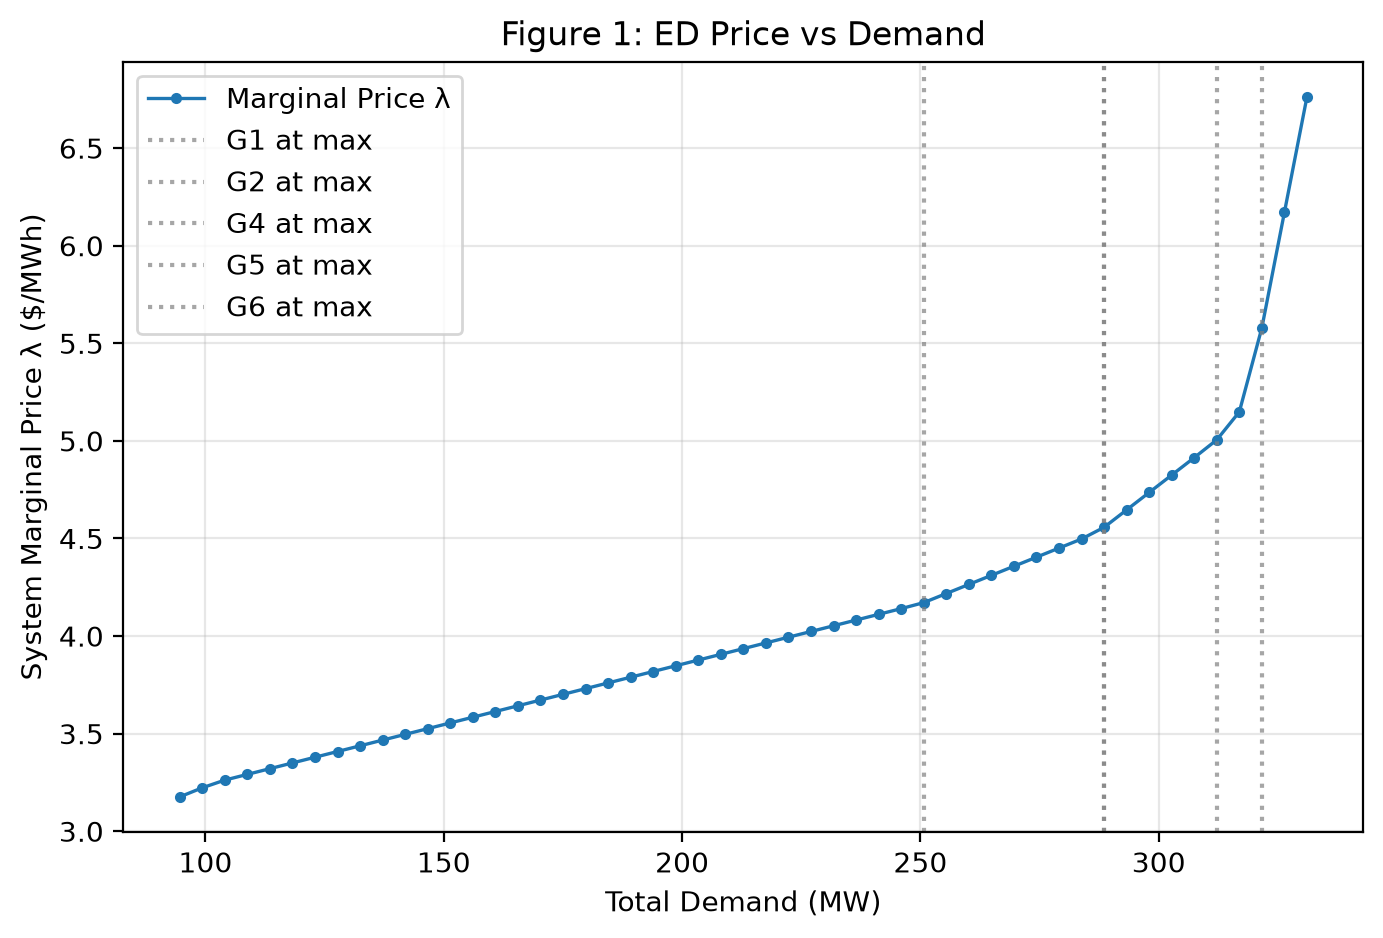
\includegraphics[width=0.85\textwidth]{fig1_price_vs_demand.png}
\caption{Economic Dispatch marginal price $\lambda$ vs.\ total demand, with generator limit transitions highlighted.}
\label{fig:price_demand}
\end{figure}

The marginal price curve exhibits distinct slope discontinuities (kinks) at specific demand thresholds where individual generators reach their maximum output capacity $P_{\max}$ and are clamped:
\begin{itemize}
    \item At $D = 260.15\text{ MW}$, Generator 4 reaches its upper limit $P_{\max, 4} = 55.0\text{ MW}$.
    \item At $D = 288.53\text{ MW}$, Generator 5 reaches $P_{\max, 5} = 30.0\text{ MW}$.
    \item At $D = 302.72\text{ MW}$, Generator 2 reaches $P_{\max, 2} = 80.0\text{ MW}$.
    \item At $D = 321.64\text{ MW}$, Generators 1 and 6 hit their respective bounds ($P_{\max, 1} = 80.0\text{ MW}$ and $P_{\max, 6} = 40.0\text{ MW}$).
    \item Generator 3 never reaches its capacity limit ($P_{\max, 3} = 50.0\text{ MW}$) within this demand range.
\end{itemize}
Whenever a generator reaches $P_{\max}$, it can no longer provide incremental energy. The system-wide incremental cost slope $\left(\sum_{i \notin \mathcal{A}} \frac{1}{2c_i}\right)^{-1}$ increases stepwise, steepening the price trajectory while preserving continuity in $\lambda$.

\subsection{Congestion Sweep and Locational Price Divergence}

Figure~\ref{fig:cost_spread} plots total operating cost and LMP spread as the line-rating scale factor is decreased from $1.000$ to $0.700$ in steps of $0.005$. Figure~\ref{fig:lmp_bus} shows the corresponding spatial distribution of LMPs across all 30 buses at selected ratings.

\begin{figure}[htbp]
\centering
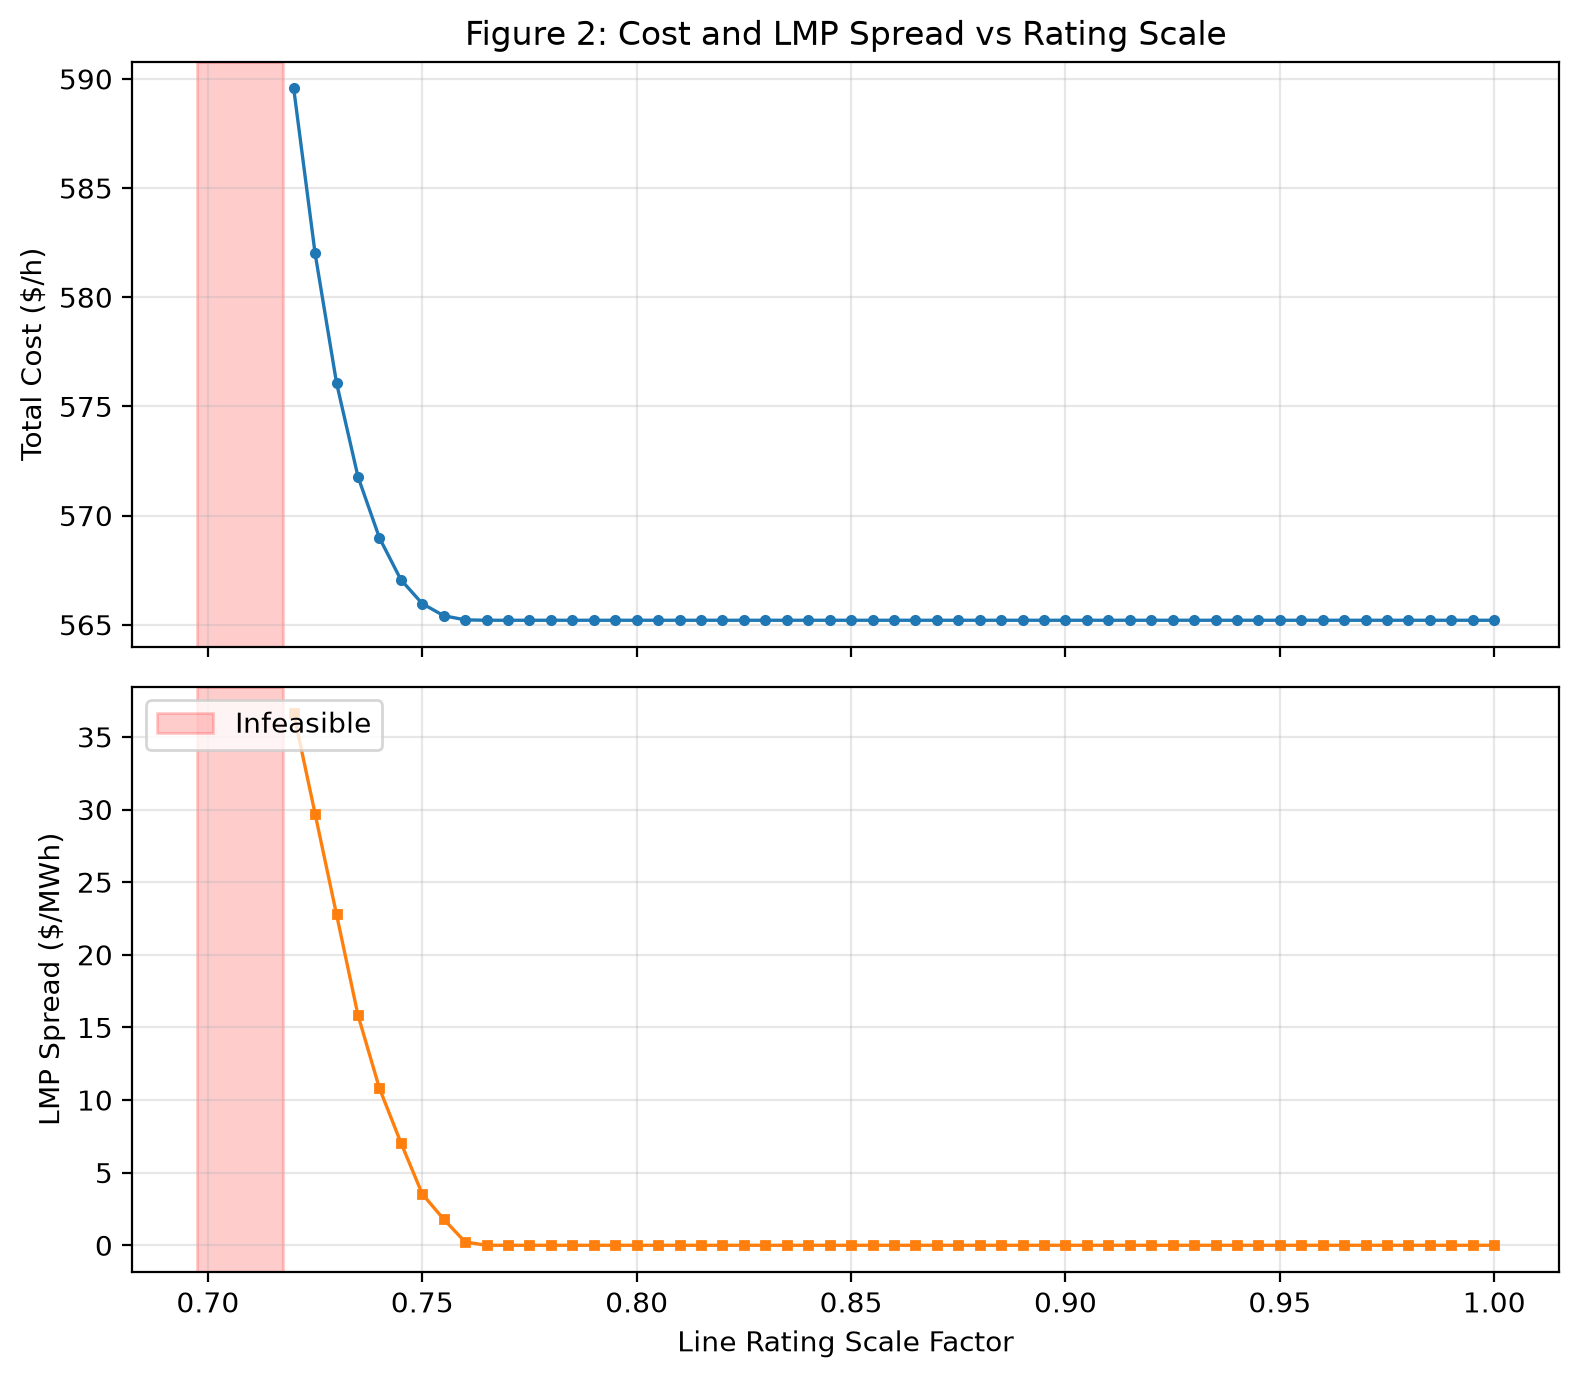
\includegraphics[width=0.85\textwidth]{fig2_cost_spread_vs_rating.png}
\caption{Total system operating cost and LMP spread vs.\ line rating scale factor.}
\label{fig:cost_spread}
\end{figure}

For ratings down to $0.765\times$, the network is completely uncongested; no line flows reach their limits, operating cost remains at $\$565.21\text{/h}$, and LMPs are uniform across all 30 buses ($\lambda = 3.7892\text{ \$/MWh}$). At rating scale $0.760$, line 6--8 becomes the first binding transmission constraint. To prevent line overload, the solver redispatches generation, causing system cost to rise to $\$565.22\text{/h}$ and LMPs to separate ($3.7885$ to $3.8117\text{ \$/MWh}$).

At rating scale $0.750$, two transmission lines bind simultaneously (branches 6--8 and 25--27). System cost increases to $\$565.97\text{/h}$, and the LMP spread widens from $3.6524$ to $7.1828\text{ \$/MWh}$. At rating scale $0.720$, four lines become constrained (branches 6--8, 15--23, 21--22, and 25--27), forcing extensive out-of-merit generation that elevates operating cost to $\$589.58\text{/h}$ and produces an extreme price spread of $3.0185$ to $39.6548\text{ \$/MWh}$.

\begin{figure}[htbp]
\centering
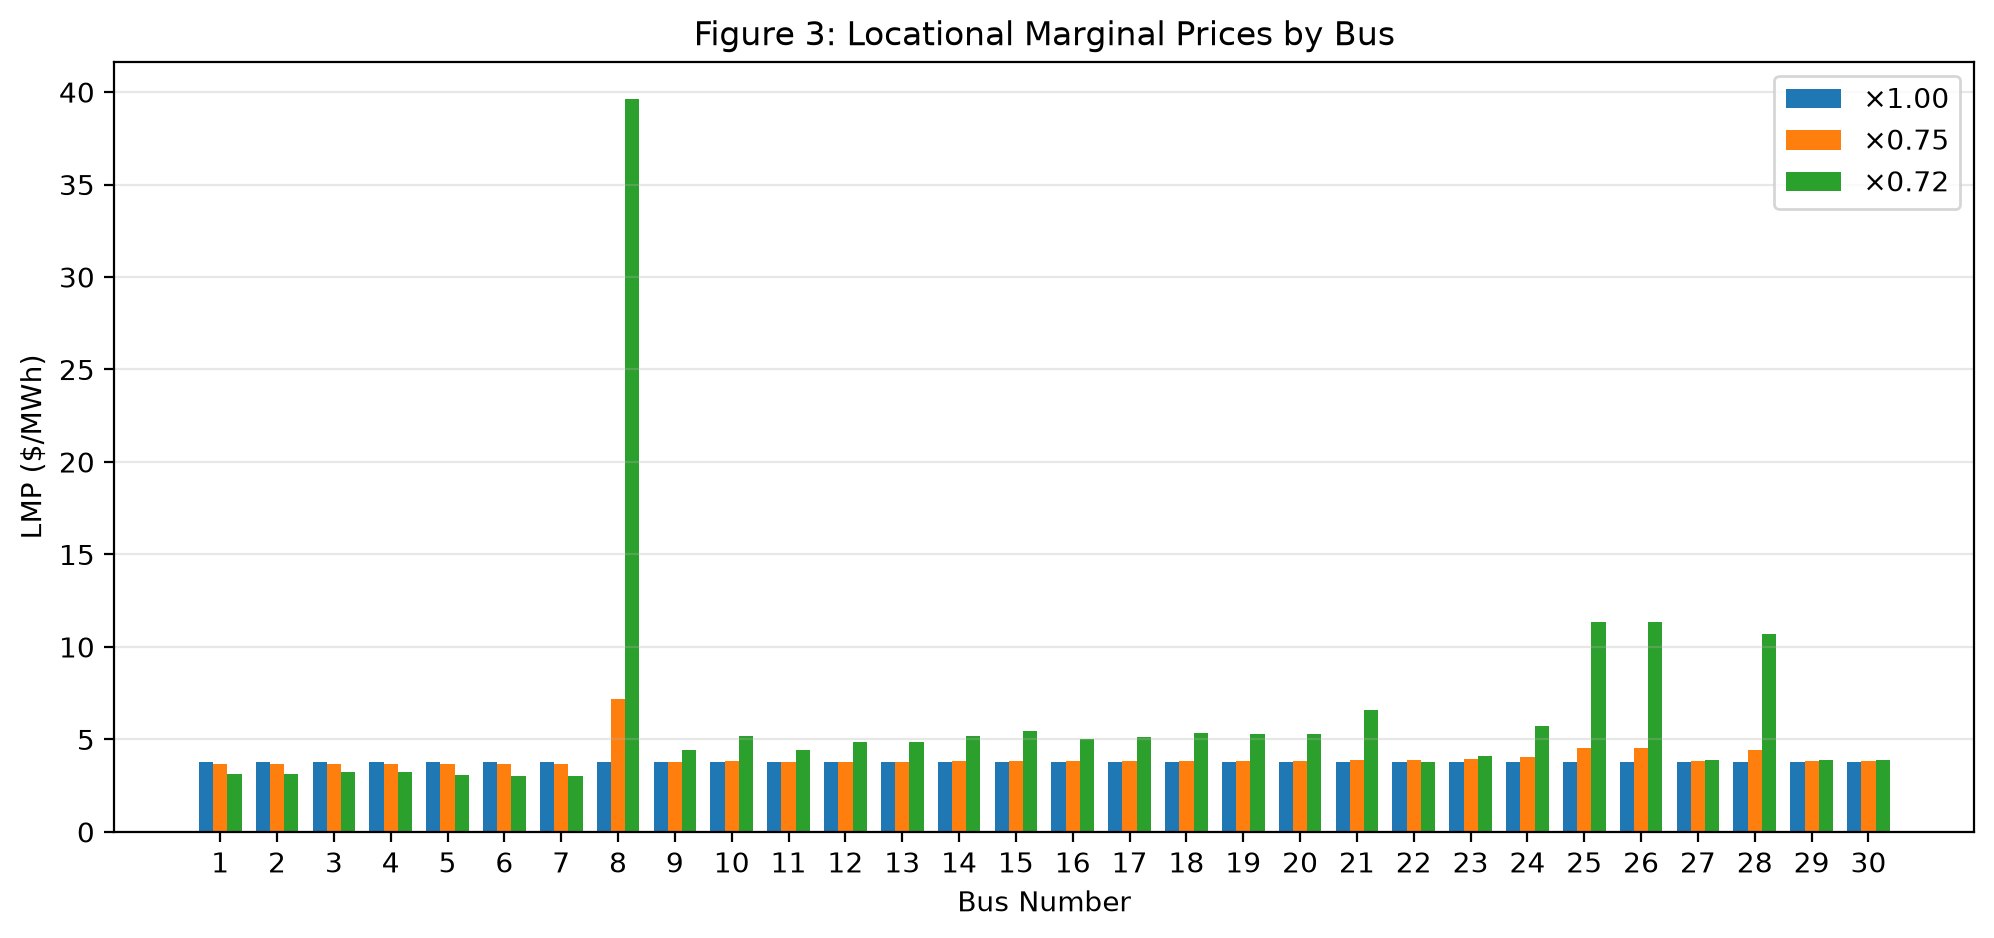
\includegraphics[width=0.95\textwidth]{fig3_lmp_per_bus.png}
\caption{Locational Marginal Prices by bus for rating scale factors 1.00, 0.75, and 0.72.}
\label{fig:lmp_bus}
\end{figure}

Bisection of the feasibility boundary demonstrates that the system becomes strictly infeasible below a line rating scale factor of $0.7167$. Below this threshold, transmission bottle-necks make it physically impossible to satisfy nodal power balances and generator capacity constraints simultaneously.

\subsection{Active-Set Convergence}

Figure~\ref{fig:convergence} displays the objective function values across iterations of the primal active-set solver when starting from non-optimal feasible initial points.

\begin{figure}[htbp]
\centering
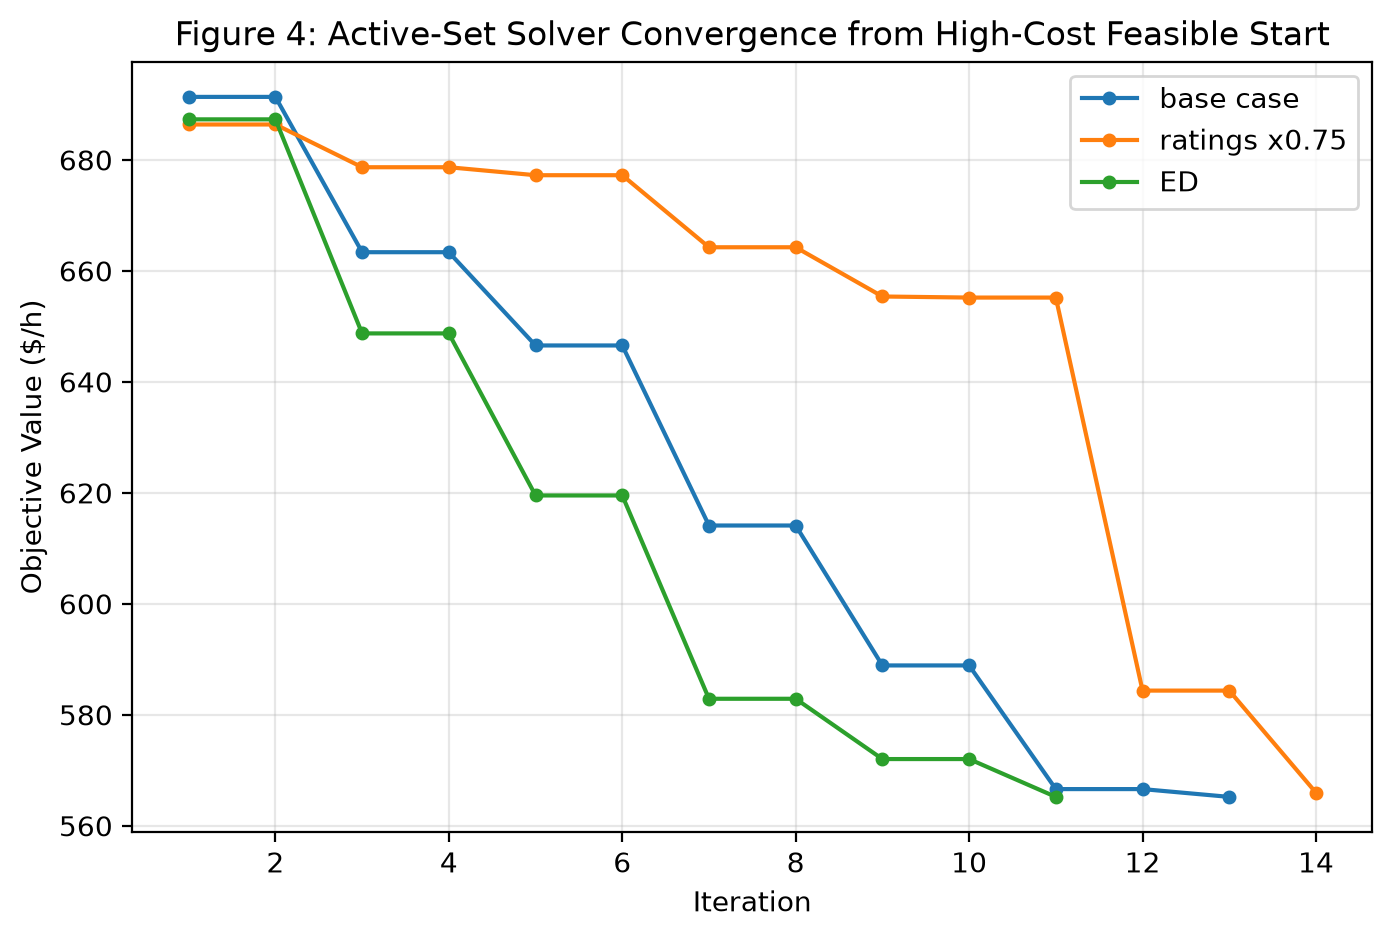
\includegraphics[width=0.85\textwidth]{fig4_active_set_history.png}
\caption{Primal active-set solver objective value per iteration from high-cost feasible initial points.}
\label{fig:convergence}
\end{figure}

In accordance with theoretical guarantees for Algorithm~16.3 \cite{nocedal2006}, the objective value decreases strictly monotonically at every iteration across all test scenarios. The uncongested base case converges in 13 iterations, the congested case ($0.75\times$) converges in 14 iterations after incorporating binding transmission constraints into the active set, and the ED case converges in 11 iterations. In each case, once the optimal active constraint manifold is identified, the subproblem step $p_k$ drops to zero, and dual multiplier non-negativity certifies optimality.
